\documentclass[]{spie}  %>>> use for US letter paper
%\documentclass[a4paper]{spie}  %>>> use this instead for A4 paper
%\documentclass[nocompress]{spie}  %>>> to avoid compression of citations

\renewcommand{\baselinestretch}{1.0} % Change to 1.65 for double spacing
 
\usepackage{amsmath,amsfonts,amssymb}
\usepackage{graphicx}
\usepackage[colorlinks=true, allcolors=blue]{hyperref}

\title{Ray-tracing a small orbital mission for soft-X-ray polarimetry}

\author[a]{Hans Moritz G\"unther}
\author[a]{Hermann L. Marshall}
\affil[a]{MIT Kavli Institute for Astrophysics and Space Research, Massachusetts Institute of Technology, Cambridge, MA 02139, USA}

\authorinfo{Send correspondence to H.M.G. (E-mail: hgunther@mit.edu)}

% Option to view page numbers
\pagestyle{empty} % change to \pagestyle{plain} for page numbers   
\setcounter{page}{301} % Set start page numbering at e.g. 301
 
\begin{document} 
\maketitle

\begin{abstract}
X-ray polarimetry is still largely uncharted territory. With the upcoming launch of IXPE, we will learn a lot more about X-ray polarization at energies above 2~keV, but so far no current or accepted mission provides observational capabilities below 2~keV. We present ray-tracing results for a small orbital mission that could be launched within NASA's Pioneer or SmallSat cost-cap to provide X-ray polarimetry below 1 keV. The design is based on the use of laterally-graded multi-layer mirrors, a concept that we have developed theoretically for the REDSoX Polarimeter\cite{redsox} and that has most components verified in the laboratory.
In this contribution, we describe a single channel orbital mission based on the same idea, but modified to the unique cost and space requirements. In particular, we use the ray-traces to define the maximum size of the dispersion gratings that can be used and to determine an alignment budget.

\end{abstract}

% Include a list of keywords after the abstract 
\keywords{ray-tracing, X-ray, polarimetry, CAT (critical angle transmission) grating, multi-layer mirror}

\section{INTRODUCTION}
\label{sec:intro}
X-rays can provide unique insight into the hot and energetic universe. While X-ray photometry and spectroscopy is now routinely performed with a number of missions, most prominently XMM-Newton and Chandra, there is no currently operating observatory to perform X-ray polarimetry and only for a single source (the Crab nebula) has there ever been a significant detection of polarized X-rays\cite{1972ApJ...174L...1N,1978ApJ...220L.117W}.
IXPE\cite{IXPE} will be launched in 2021 and provide this capability for X-rays above 2~keV, but there is still no instrument in sight for soft X-ray polarimetry. Yet, a range of open science questions for several classes of astrophysical sources can only be answered with soft X-ray polarimetry.


\section{MISSION OVERVIEW}
Over the years, we have developed and refined a design for a soft X-ray polarimeter, called ``REDSoX'', which is based on reflection of a multi-layer mirror.  
Details of the REDSoX design are discussed in Ref.~\citenum{redsox}, more details of ray-trace calculations are presented in Ref.~\citenum{redsoxtrace}.
In short, X-rays are focussed into a converging beam using a mirror. Beyond the mirror, the photons encounter critical-angle transmission (CAT) gratings. A fraction of the photons passes through (0th order) onto an imaging detector, which can be used to confirm the accuracy of the pointing and provide an X-ray spectrum with the intrinsic energy resolution of the detector. Most photons however, are diffracted. By selecting the blaze angle (the angle between the grating normal and the direction of the incoming photons), we can optimize the fraction of photons diffracted into the zeroth order. Photons of longer wavelength are diffracted further and thus hit the focal plane further away from the direct image than photons with a shorter wavelength. In the focal plane, a multi-layer mirror is located. The thickness of the layers varies with position (``laterally graded'') and is chosen such that every photon interacts with the mirror at a position where the mirror spacing matches Bragg condition for photons of that wavelength. The mirror is tilted by about 45 degrees with respect to the incoming photons, and thus only photons with one polarization direction are reflected, while photons with a perpendicular polarization are absorbed. A CCD detects the reflected photons. The requirement to match the photon position to the Bragg peak on the multi-layer mirror sets a limit to the width of the mirror point-spread function in the dispersion direction. We achieve this by sub-aperturing, i.e.\ we use only wedge-shaped mirror modules and not full circles.

Measurement at several angles are required to reconstruct the polarization fraction and angle. In our design, this can be achieved with a single multi-layer mirror, if the entire instrument rotates (either continuously or in steps) or with two or three channels, each with its own sub-aperture, multi-layer mirror and detector.

REDSoX is designed as a sounding rocket payload with very short exposure times, but loose mass and space requirements. In this paper, we present ray-traces for a variant of the REDSoX design optimized for a small orbital mission, e.g.\ in NASA's Astrophysics Pioneer or SmallSat program. Compared to REDSoX, we need to shorten the focal length to fit the mission into the envelope of a secondary payload and reduce the area covered by the mirrors; on the other hand, exposure times can be much longer. While a sounding rocket gives only a few minutes of X-ray observing time, we can integrate for months in an orbital missions. Much of the trades and studies done for REDSox\cite{redsoxtrace} are applicable here, too, just with different numbers for the focal length, but others are unique to this design, e.g.\ the much longer exposure times require a much more careful estimate of the background that is picked up in the detectors.
While the sounding rocket REDSoX is designed with three polarization channels, an orbital mission with much longer exposure times can work with just one or two channels because lower effective areas can be offset by longer exposure times.

In this work, we consider a system with a focal length of just 1.25~m and a single polarimetry channel. An overview of the design is shown in Figure~\ref{fig:3d}. This matches our submitted Astrophysics Pioneer proposal and represents the simplest possible instrument to measure soft X-ray polarimetry. It is easy to extent this design by adding another polarimetry channel for redundancy, increased effective area, and the opportunity to measure fast changes in the polarization (since two polarization directions are observed simultaneously, instead of rotating the instrument). 

   \begin{figure} [ht]
   \begin{center}
   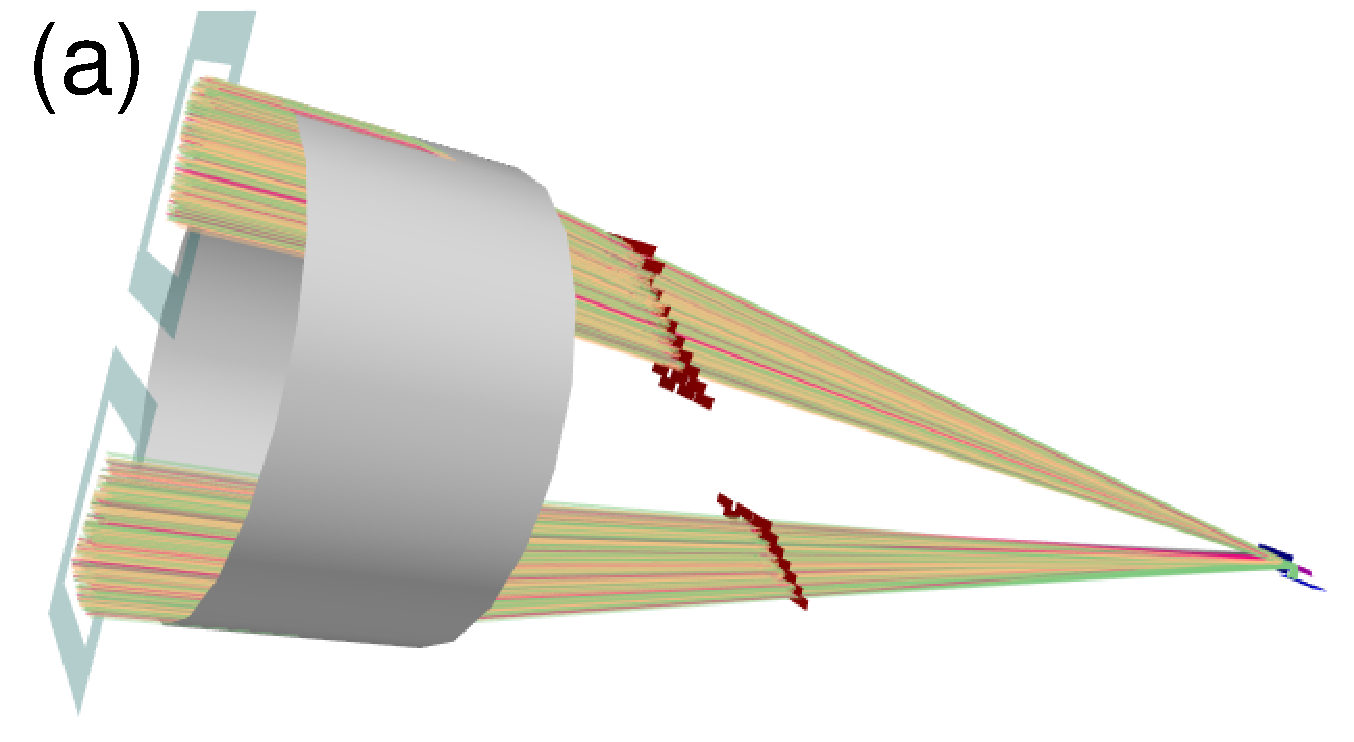
\includegraphics[height=5cm]{3D.pdf}
   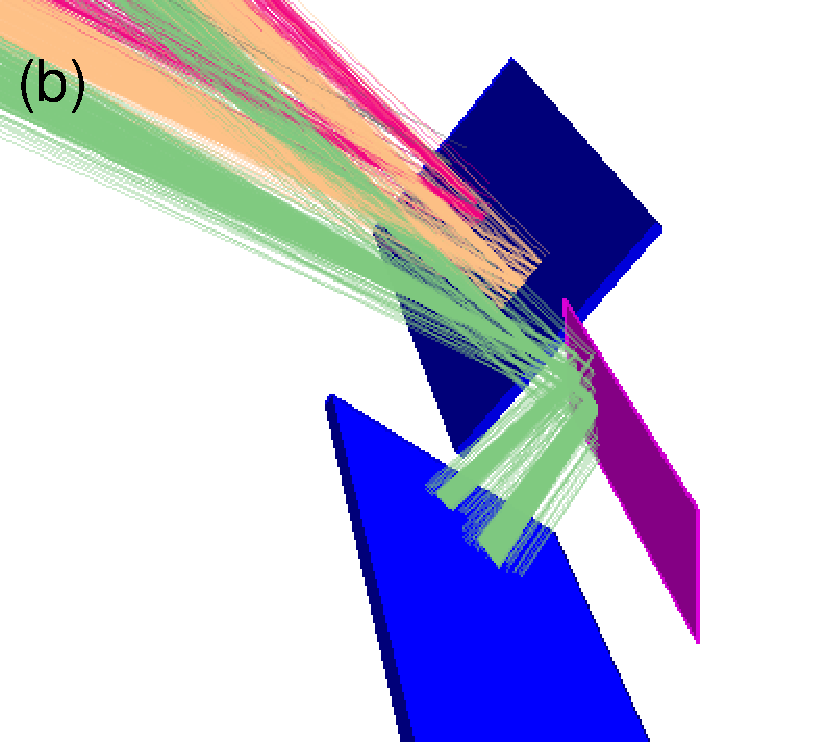
\includegraphics[height=5cm]{3Ddetector.pdf}
   \end{center}
   \caption
   { \label{fig:3d}3D rendering of the instrument design and a ray-trace for monoenergetic rays of 0.3~keV. The ray-trace setup makes some simplifications. In particular, the mirror is not modeled in 3D, but approximated by a 2D lens. In the 3D view, the position of the mirror modules is just indicated schematically by a cylinder that has the same radius as the outermost mirror surface. This is a monochromatic simulation with photon energies of 0.3 keV. Only rays that are detected in the end are shown and rays are colored according to the grating diffraction order. The zeroth order is shown with gray rays, the first order with green rays. The green rays bounce of the multilayer-mirror (purple) because they hit a detector (blue). The  second detector (also blue) images the zeroth order, but also photons diffracted into order -1. \emph{panel a:} View of the full instrument. The astrophysical source is located along the top left. Rays are shown starting at the entrance aperture. \emph{panel b:} Zoom into the focal plane with multi-layer mirror (purple) and two detectors (blue). 
}
   \end{figure}

Figure~\ref{fig:3d} shows a ray-trace through our one-channel system. All rays i the figure have the same energy (0.3~keV). Because the mirrors deliver a converging beam, the angle between ray and multi-layer mirror spans a range of incident angle. Thus, rays need to reach the multi-layer mirror at slightly different angles to fullfill the Bragg condition. In panel (b) of the figure, it can be seen that the rays fall into two groups depending on if they pass through the upper or lower sector of gratings. See Ref.~\citenum{redsox} for a derivation of the grating position depending on the multi-layer mirror gradient and position.

\section{SETUP FOR RAY-TRACES}
We perform a geometric ray-trace with the MARXS code, which follows individual rays through the system from the entrance aperture to the detector. Simulations are performed with MARXS 1.2\cite{marxs,marxs1.2}. MARXS is
written in Python and available under the GNU license v3. The code is available on github\footnote{\url{https://github.com/chandra-marx/marxs}}. Specific code for the simulations of the instrument shown here is also available\footnote{\url{https://github.com/X-raypol/ray-trace}}; we used the version with commit hash 13b10be. More details on the code can be found in proceedings describing its application for other missions\cite{10.1117/12.2525814,10.1117/12.2312678}.

Every simulation contains some simplification of reality, e.g., because certain aspects of the design are not known yet, laboratory data about performance must be extrapolated, or simply because computational cost puts limits on how many photons can be run through a simulation. Our simulations are set up with a relatively simplistic mirror model. Instead of a three dimensional structure, the mirror is implemented as plane perpendicual to the optical axis. When rays intersect the plane, their directions are modified as if they pass a perfect lens. In the next step, additional scatter in the plane of reflection is added. For each ray, the scattering angle is drawn from a Gaussian distribution, where the width of the distribution is tuned to achieve a PSF size that matches the PSFs measured or exepcted for the type of mirror used. We use 12 arcsec for the $\sigma$ of the Gaussian.

Our instrument uses CAT gratings manufactured from Si wafers at the MIT Space Nanotechnology Laboratory
\cite{Heilmann:11,doi:10.1117/12.2188525,10.1117/12.2314180,10.1117/12.2529354}. The grating efficiency of these gratings is calculated based on simulations and verified in the laboratory; a table if efficiencies is an input to our simulations. The high aspect-ratio grating bars are 4~$\mu$m deep and supported by an L1 support structure running perpendicular to the grating bars themselves and the entire membrane (bars and L1) is mechanically stablized by an L2 support structure, which is 0.5~mm deep. Absorption and diffraction of photons by the L1 and L2 support structures is included in our simulations. The grating membrane is surrounded by a 0.5 mm wide frame of solide Si for handling and glued into a grating holder.

Laterally graded multi-layer mirrors can be made from a variety of materials. We use a Cr/Sc mirror, because this combination of material promises a good reflectivity in the bandpass of interest. The detectors will be CCD ID-94 detectors produced by Lincoln Labs, we use the quantum efficiencies measure for Suzaku CCDs\cite{2007PASJ...59S..23K} for our ray-traces.

\section{PERFORMANCS}
\label{sect:performance}
The main cahracteristics are of a polarimeter are its effective area and the modulation factor.
\subsection{Effective area and modulation factor}
In order to determine the modulation factor, we perform simulations for a source that is 100\% polarized. Then, we turn the pointing of the instrument on the sky in small steps so that we can build up the modulation curve. From this curve, the total modulation of the signal can be calcualted as $\frac{T-B}{T + B}$, where $T$ is the maximum of the curve and $B$ is the minimum. Curves for effective area and modulation are shown in figure~\ref{fig:aeff}.
   \begin{figure} [ht]
   \begin{center}
   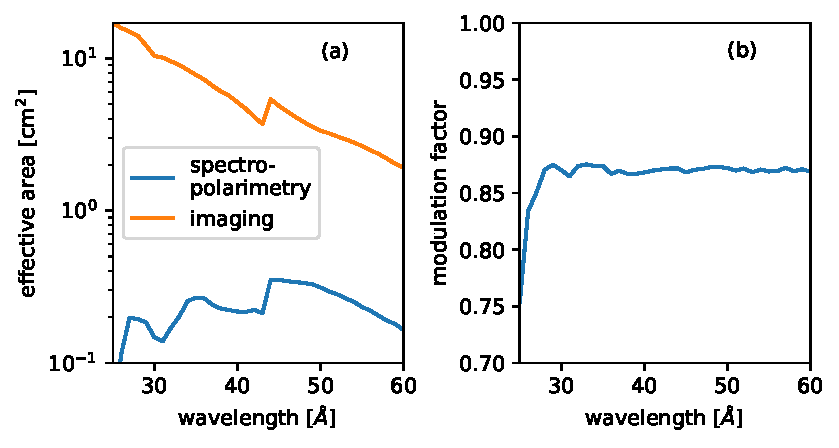
\includegraphics[height=5cm]{aeff.pdf}
   \end{center}
   \caption
   { \label{fig:aeff} \emph{panel a}: Effective area. CCD~1 detects the polarized signal, CCD~0 the zeroth order. Because CCD 1 observed the signal of the multi-layer mirror, the effective area is much lower than in the CCD~0. \emph{panel b:}: modulation factor.
}
   \end{figure}

\subsection{How does an observation look?}
Since we have only a single polarimatery channel, we have to rotate the instrument on the sky to cover enough range in rotation angles to sample all possible polarization directions. We show simulations with the spectrum and flux of Mk 421 assuming the source is fully polarized. In reality, the polarization fraction is going to be $<1$ and might depend on energy. Of course, we can simulate those scenarios, too, but the point here is to show how the data works in principle, so we pick the easiest scenario.

We simulate two observations with different polarization angles on the sky, which are chosen such that the first angle gives the maximal signal and the second one the minimal signal on the polarization channel. In a real observation, that angle is not known a-priory and the instrument needs to be rotated continuously or observe at at least three angels to be able to uniquely derive the polarization fration and angle from the polarization channels alone. Using the zeoths order as well, observations at two angles are sufficient.

\section{TRADES}
\label{sect:trades}

\subsection{Bending gratings}
The grating efficiency of CAT gratings changes with the blaze angle. If the blaze angle is small, i.e.\ the rays hit the grating parallel to the surface normal, then many rays will pass ``straight through'' to the zeroth order. Higher blaze angles favour higher orders. PiSox is designed for the blaze angle of 0.8 degree to maximise the number of photons that are diffracted into the first order where they will hit the multi-layer mirror at the blaze peak. We position the gratings such that a ray hitting the grating center has a blaze angle of 0.8 degrees. Since the gratings are located in a converging beam the blaze angle for rays hitting a flat grating near the edges is different from the nominal blaze angle. Fewer photons are diffracted into the first order and the effective area is reduced.

This can be corrected by bending the gratings. If the grating surface follows a cylinder with a radius of curvature that matches the distance of the grating from the focal point, that effect can be almost entirely be compensated (Figure~\ref{fig:curvature}. The axis of that cylinder is parallel to the cross-dispersion direction. In other words, the grating is curved along the long side. On the other hand, bending almost every grating with a different radius of curvature increases the complexity and thus cost and schedule risk dramatically. Here, we study four different scenarios:
\begin{itemize}
    \item Gratings are flat.
    \item All gratings are bend with the same radius which is chosen to be close to the average distance beween grating and focal point.
    \item We use two different radii of curvature for the upper and lower part of the grating staircase.
    \item Each grating is curved individually.
\end{itemize}

   \begin{figure} [ht]
   \begin{center}
   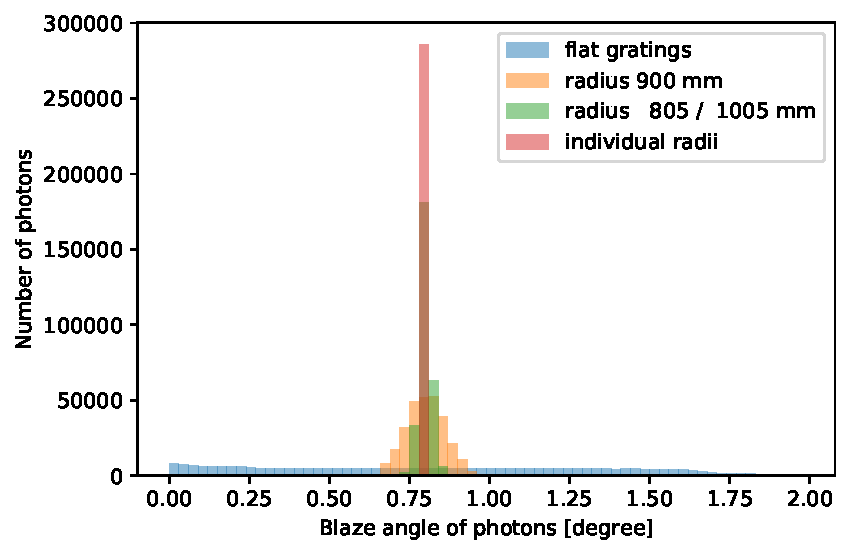
\includegraphics[height=5cm]{curvature.pdf}
   \end{center}
   \caption
   { \label{fig:curvature}Distribution of blaze angles (angle between incoming ray and local normal to the grating surface) for different radii of bend CAT gratings.
}
   \end{figure}

\begin{table}
  \caption{effective area in the imaging and polarimatery channel for a representative energy of 0.277 keV}
  \label{tab:curvature}
\begin{center}
\begin{tabular}{c|c|c}
scenario & imaging & polarimetry \\
& $\mathrm{cm^{2}}$ & $\mathrm{cm^{2}}$ \\
\hline\hline
flat gratings & 5.43 & 0.145 \\
radius 900 mm & 4.99 & 0.210 \\
radius   805 /  1005 mm & 4.99 & 0.214 \\
individual radii & 4.97 & 0.213 \\
\end{tabular}
\end{center}
\end{table}
Table~\ref{tab:curvature} shows simulated effective areas at a representative energy for all four scenarios.
Flat gratings have the best imaging performance, but severely reduce the effective area of the more important polarimetry channel. There is little performace difference between the different bending options studied here, so we conclude that the simplest option (all gratings have the same curvature) should be the baseline design for our instrument.

\subsection{Grating dimensions}
We use a baseline design with rectangular CAT gratings with edgle lengths of 30 mm and 10 mm, where the long edge is parallel to the dispersion direction. In this trade, we test the choice of 10 mm width for the corss-dispersion direction. CAT gratings can be manufactured in larger sizes, but the ideal surface on which the gratings need to be placed is saddle-shaped. On the other hand, the design of the gratings requires the grating normal to be roughly perpendicular to the incoming rays. If the angle between ray and grating becomes large, then the support structures that hold the grating bars in place, in particular to so-called L2 support structure that is 0.5~mm deep, would cast large shadows and thus reduce the effective area. The grating membranes are fixed to the metal grating holder, which in turn is mounted to a larger mechanical structure. All these block some fraction of the area and thus reduce the number of rays that make it through to the detector.

So, there are two competing effects: On the one hand, larger gratings reduce the number of and thus area lost to these mounting structures; on the other hand, we have the constrained that the CAT grating normals are close to the direction of the incoming rays. Thus, the larger the grating, the more do the regions on the edges deviate from the surface on which the diffraction should happen. Instead, some rays hit the grating where it is located "above" the theoretical surface, and some "below". In the the first case, photons are diffracted too far, on the latter to little. Both can cause photons to arrive at the ML mirror at a position that does not match the Bragg peak for their wavelength.

Figure~\ref{fig:width} shows the effective area in simulations with different CAT grating sizes. For grating holders with wide frames the ideal width is between 5 and 10 mm. Since the total effective area plateaus in that range, we can see that 10 mm wide gratings are a good choice for the design baseline. Narrower gratings can achieve te same effective area, but at a larger cost and complexity. 
\begin{figure} [ht]
  \begin{center}
    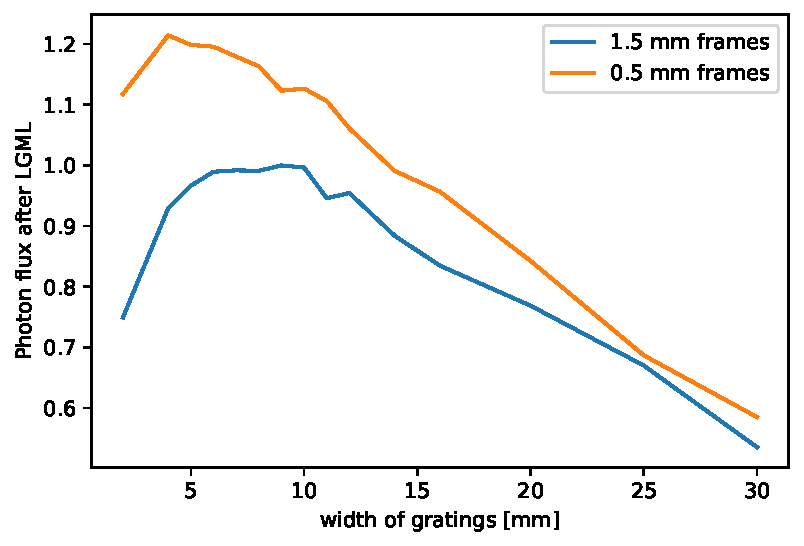
\includegraphics[height=5cm]{catdimensions.pdf}
  \end{center}
  \caption
      { \label{fig:width}Effective area for an instrument filled with CAT gratings of different dimensions. In all simulations, th CAT gratings are 30 mm long in dispersion direction, but the width of the grating in cross-dispersion direction differs. When using larger gratings, there is less obscuration by frames and grating holders, but gratings deviate more from the ideal surface. The figure shows that gratings with dimensions of $30\times10\;\mathrm{mm}^2$ perform best.
}
\end{figure}

\section{ALIGNMENT AND ERROR BUDGET}
\label{sect:align}
When the physical hardware for a mission is put together, nothing is perfect. Parts and pieces will always differ slightly in form, shape, and position from the locations assigned to them in the abstract design model. Ray-tracing is one useful method to study how much such misalignments will impact the performance of the instrument and thus to develop a table of alignment requirements. The looser the requirement can be, the cheaper and faster the process is. On the other hand, if the ray-tracing shows that certain elements need to be positioned very precisely, specific alignment procedures and tests might have to be developed.

For each alignment parameter, we study six degrees of freedom (three translantions and three roations). In practice, misalignments happen in all six degrees of freedom for all parts of the instrument at the same time. However, computational limitations prohibit us from exhaustively exploring the full parameter space. Instead, as a first phase, we treat PiSoX as a hirachical collection of many elements (mirror shells, mirror module, CAT gratings, CAT grating assembly, all of which combine into the optics module etc.). We perform simulations for about a dozen elements and for each parameter we typically run simulations for 10-20 values. The full parameter space would thus require $20^{6*12}=5\times 10^{93}$ simulations. Instead, as a first step, we set up a perfectly aligned instrument and then vary one parameter for one element or one group of elements (e.g. the "x" position of all gratings) at a time. Note that even a perfectly aligend instrument has some limitations that are inharent in the design, such as optical abberations. We step through diffferent values for each parameter, keeping all other alignments perfect, and run a simulations with 100,000 photons for each step. We inspect the results from simulations and select a value for the accpetable misalignment in each degree of freedom, e.g. the value where the effective area of the channel degrades by no more than 10\%. Selecting the exact value is a trade-off with engeneering concerns. In some degrees of freedom, the alignment may be easily reached by machining tolerances and thus we can chose a number that causes only a negligible degradation of performance, while in other cases, reaching a certain alignment might be very costly and thus we want to set the requirements for this parameters as loosely as possible.

In many cases, the effects of different misalignments will just linearly add up, in others they may cancel each other out to some degree or combine multiplicatively. In future work step, we will investigate misalignments for all parameters simulataneously, but instead of exhaustivly covering the entire parameter space, we perform simualtions only for the table of aligment requirements developed in Step 1.

For the purpose of developing the error budget, there are other design parameters that are not technically related to mechnical aligment, but impact the performce in a similar way and can be analyzed with the same ray-trace setup. One example is the pointing jitter, which describes how uncertainties in the instrument pointing on the sky degrade the instrument performance. If the pointing direction on the sky jitters with time, photons will not always arrive on-axis. This is somewhat similar to a misaligned optics module.

In this section, we run simulations varying one degree of freedom at a time and present results in three different kinds of plots: First, there are parameters that are not mechanical misalignments, such as the pointing jitter. Figures showing the results of these simulations have a blue background. Simulations for mechanical misalignments come in two flavors. Either an entire set of objects is moved determinsitically (e.g. all gratings in the grating assembly are moved 1 mm to the right) or a number of objects are moved randomly (e.g. all gratings in the grating assembly are moved along the $x$-axis, but for each grating a new number is drawn from a Gaussian distribution with $\sigma=1$ mm). The first case is shown with a gray background, the latter case is shown with a pink background. Results for all mechnical tolerancing are shown as sets of six plots. The upper row presents results from translations along the $x$, $y$, and $z$-axis, the bottom row rotations. The center of the rotation is typically the centor of an element. If other centers are chosen, this is discussed in the text. The coordinate system for the instrument places the optical axis along the $z$-axis with photons coming in from $z=+\infty$. The origin of the coordinate system is at the nominal focal point of the mirror system. The dispersion direction of the gratings is along the positive $y$-axis. Thus, the long axis of the ML mirror is also parallel to the $y$-axis.

\subsection{Pointing and mirror}
\begin{figure} [ht]
  \begin{center}
    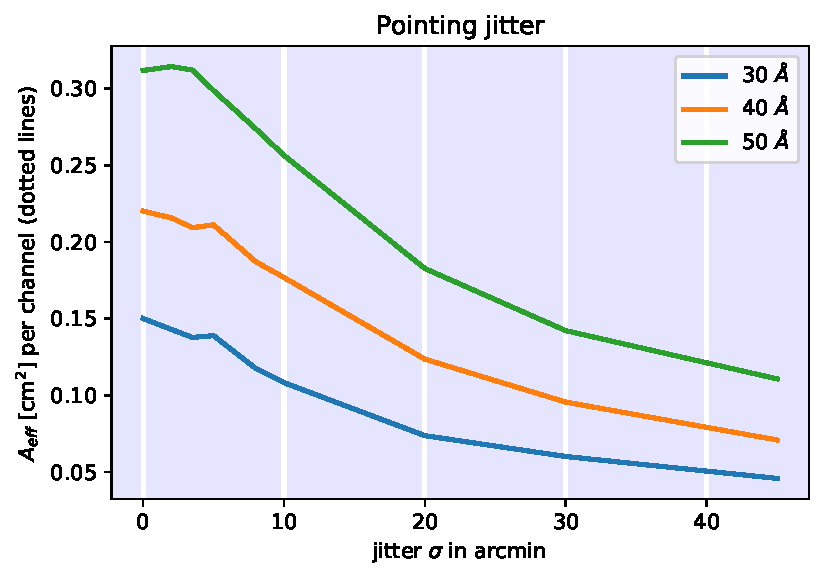
\includegraphics[height=5cm]{jitter.pdf}
  \end{center}
  \caption
      { \label{fig:jitter}Change of effective area with increasing pointing jitter. 
}
\end{figure}

Figure~\ref{fig:jitter} shows simulations using an unsteady pointing. The average pointing direction is on-axis, but the pointing jitters around that. For each photon, the true pointing direction is drawn from a Gaussian with the $\sigma$ given in the figure. This jitter represents uncertainty in the pointing, which can come from different sources, such as limited resolution of the star trackers, motion of the pointing within the time period of reading out the star trackers or integetration time of the zero-order image (if used to determine the target coordinates) or the spacecraft not correcting a pointing drift fast enough.

The effective area $A_{\mathrm{eff}}$ drops with increasing jitter, because the diffracted photons do not hit the ML at the position of the Bragg peak when the target is not at a nominal position, and thus the reflectivity is lower. The drop becomes important for a jitter above a few arcminutes. Mispointing along the direction of diffraction has a much stronger effect than perpendicular to it. This is investigated in figure~\ref{fig:offset_point}.

\begin{figure} [ht]
  \begin{center}
    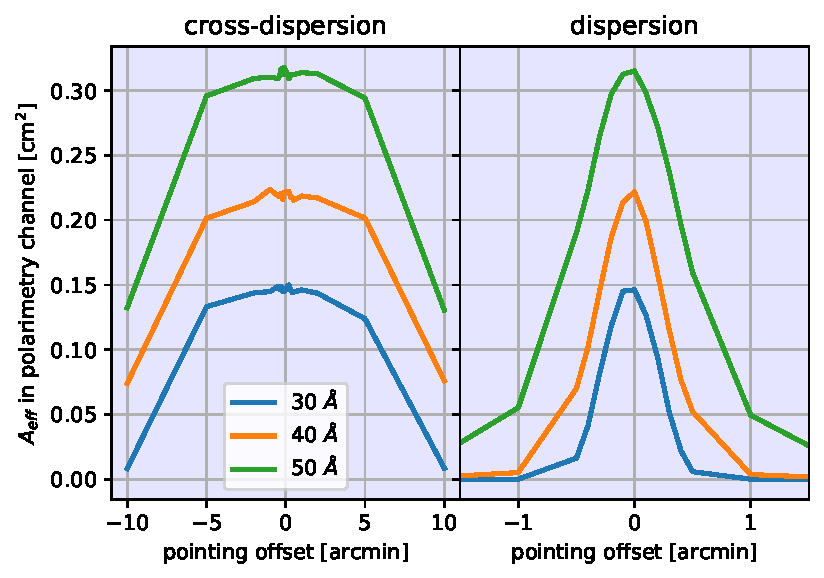
\includegraphics[height=5cm]{offset_point.pdf}
  \end{center}
  \caption
      { \label{fig:offset_point}Change of effective area for observations where the target is positioned offset from the nominal pointing direction. 
}
\end{figure}

The modulation factor changes only marginally when the source is observed offset from the nominal position. However, as explained for the simulations with the pointing jitter above, the effective area drops dramatically when the source  moves along the axis of the ML, because that means that photons will no longer arrive at the position where the spacing of the ML matches the required number given the angle and wavelength of the photon. Because photons with a longer wavelength are more dispersed, they are more effected.


\subsection{CAT gratings}
\begin{figure} [ht]
  \begin{center}
    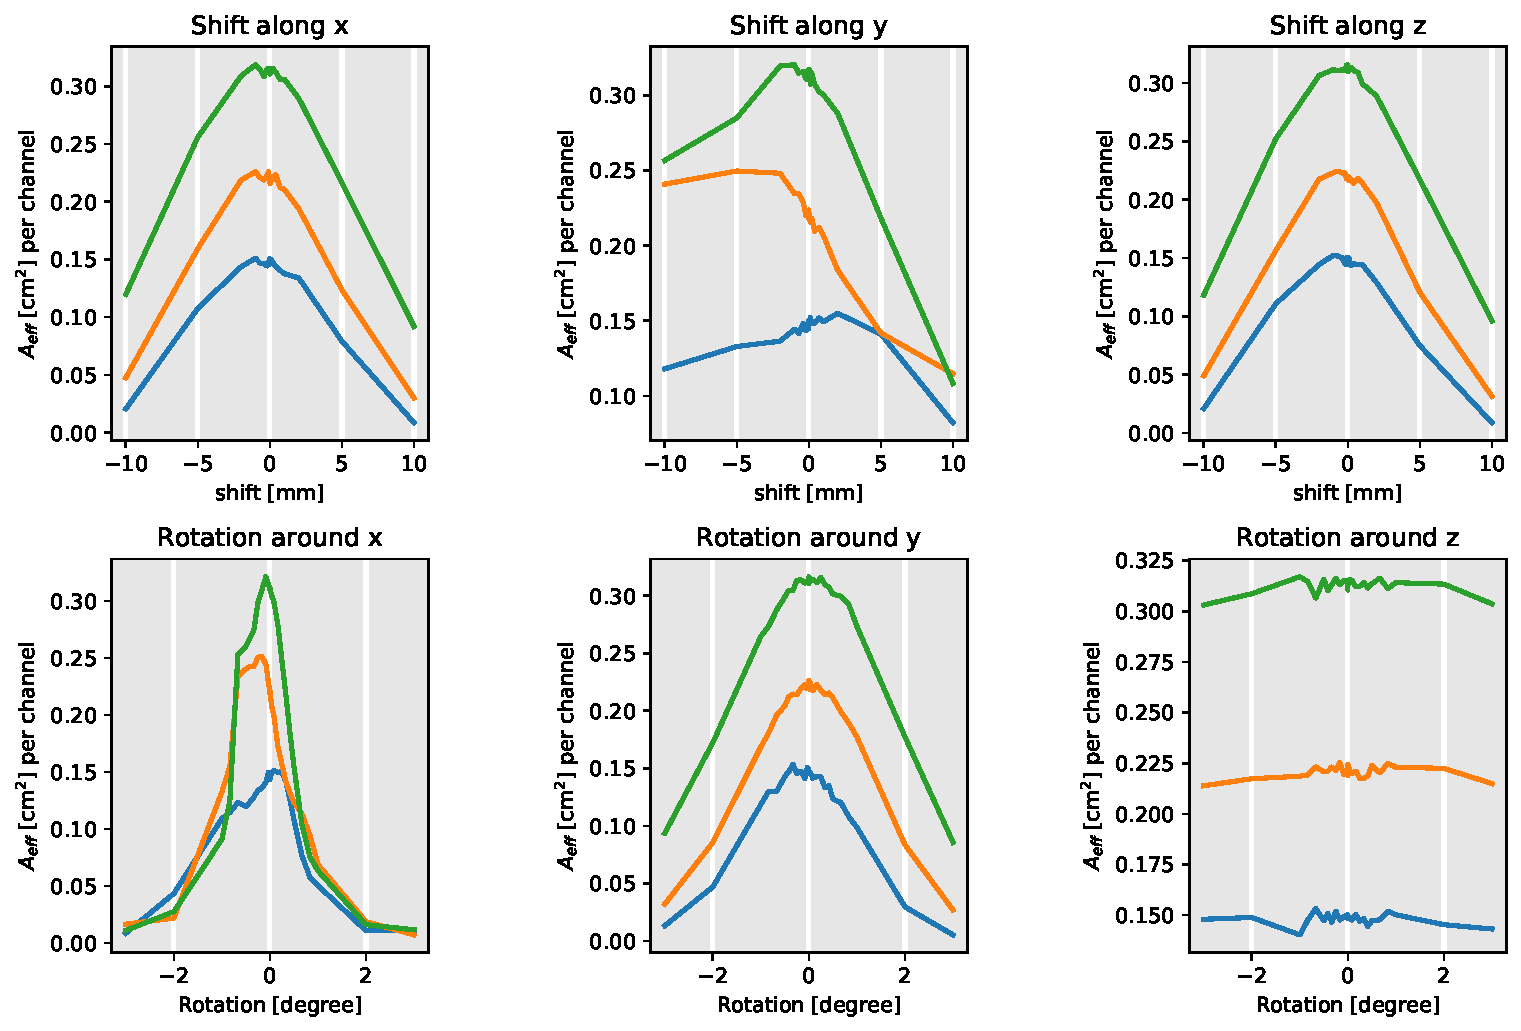
\includegraphics[height=8cm]{CAT_global.pdf}
  \end{center}
  \caption
      { \label{fig:CAT_global}Change of effective area for globally misaligned CAT grating module. 
}
\end{figure}
Figure~\ref{fig:CAT_global} shows simulations that move the CAT grating modules as a whole, i.e.\ translation in $z$ means that all gratings of both sectors are moved up or down together. This particular case changes the distance between the gratings and the focal plane and thus photons will hit the ML mirror on a different location. Changes of more than a few mm will cause the photons to miss the position of the Bragg peak on the ML mirror and thus reduce $A_{\mathrm{eff}}$. The layout is insentitive to translations in $y$ (along the dispersion direction). This is the long direction of the CAT gratings and CAT gratings are tilted only ever so slightly, so that the point of intersection is essentially constant. $A_{\mathrm{eff}}$ only begins to drop, when gratings are moved so far that some fraction of the beam no longer hit a grating. A shift along $x$ is a shift along the stair-stepped direction. Shifts along $x$ reduce $A_{\mathrm{eff}}$ for the same reason that the layout is stair-stepped in the first place: Since photons come in at a different angle, they need to be diffracted at a different distance from the ML to hit the ML mirror at the Bragg peak.

For the rotation simulations, the origin of the rotation is the point where the optical axes intersects the "stair" surface on which the gratings are positioned. Of all the rotations, only rotations around the $y$ direction (the dispersion axis) have limits tighter than a degree or so, because rotation around $y$ changes the $z$ position of the gratings, so the effect is similar to a translation in $z$.

\subsection{CAT gratings}
\begin{figure} [ht]
  \begin{center}
    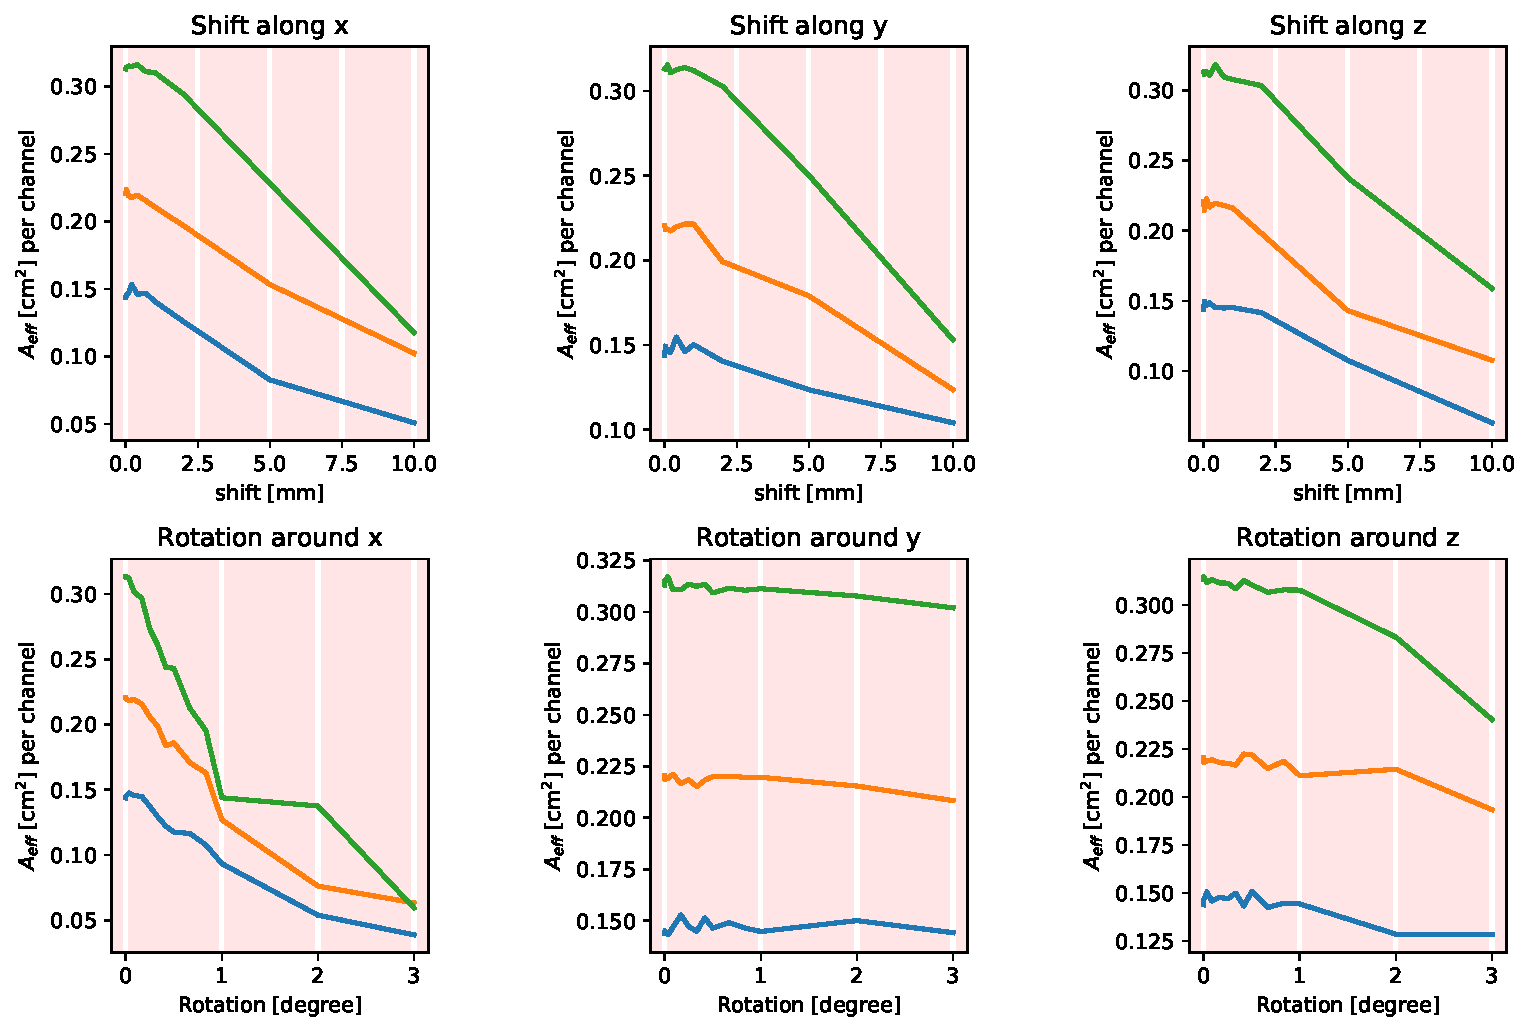
\includegraphics[height=8cm]{CAT_individual.pdf}
  \end{center}
  \caption
      { \label{fig:CAT_individual}Change of effective area for CAT gratings misaligned with respect to each other.
}
\end{figure}

Figure\ref{fig:CAT_individual} presents simulations where individual CAT gratings are moved with respect to their nominal position on the CAT gratings assembly, i.e. where the grating holders are not positioned correctly. All translations allow $1\sigma$ errors of a few mm, which is much larger than the size of the holder the gratings are placed in. This is a trivial constraint. Similarly, only rotations around $x$ (the short axis of the gratings) is tighter than 2 degrees. Rotations around $x$ makes the incoming photons hit the CAT gratings at an angle different from the design blaze angle and reduce the fraction of photons that are dispersed into the first order. Since photons in other orders are not reflected from the ML mirror onto the detector, this reduces the $A_{\mathrm{eff}}$ of the system. Longer wavelengths drop faster. To keep the loss of $A_{\mathrm{eff}}$ below 10\%, the gratings need to be positioned within 10 arcmin of the nominal rotation angle.

A change in the period of the gratings will also diffract photons to the wrong locations, but the lithography process used to manufacture the gratings gives a repeatability of the grating period that is orders of magnitude better than the PiSoX requirement.

\subsection{ML mirror}
\begin{figure} [ht]
  \begin{center}
    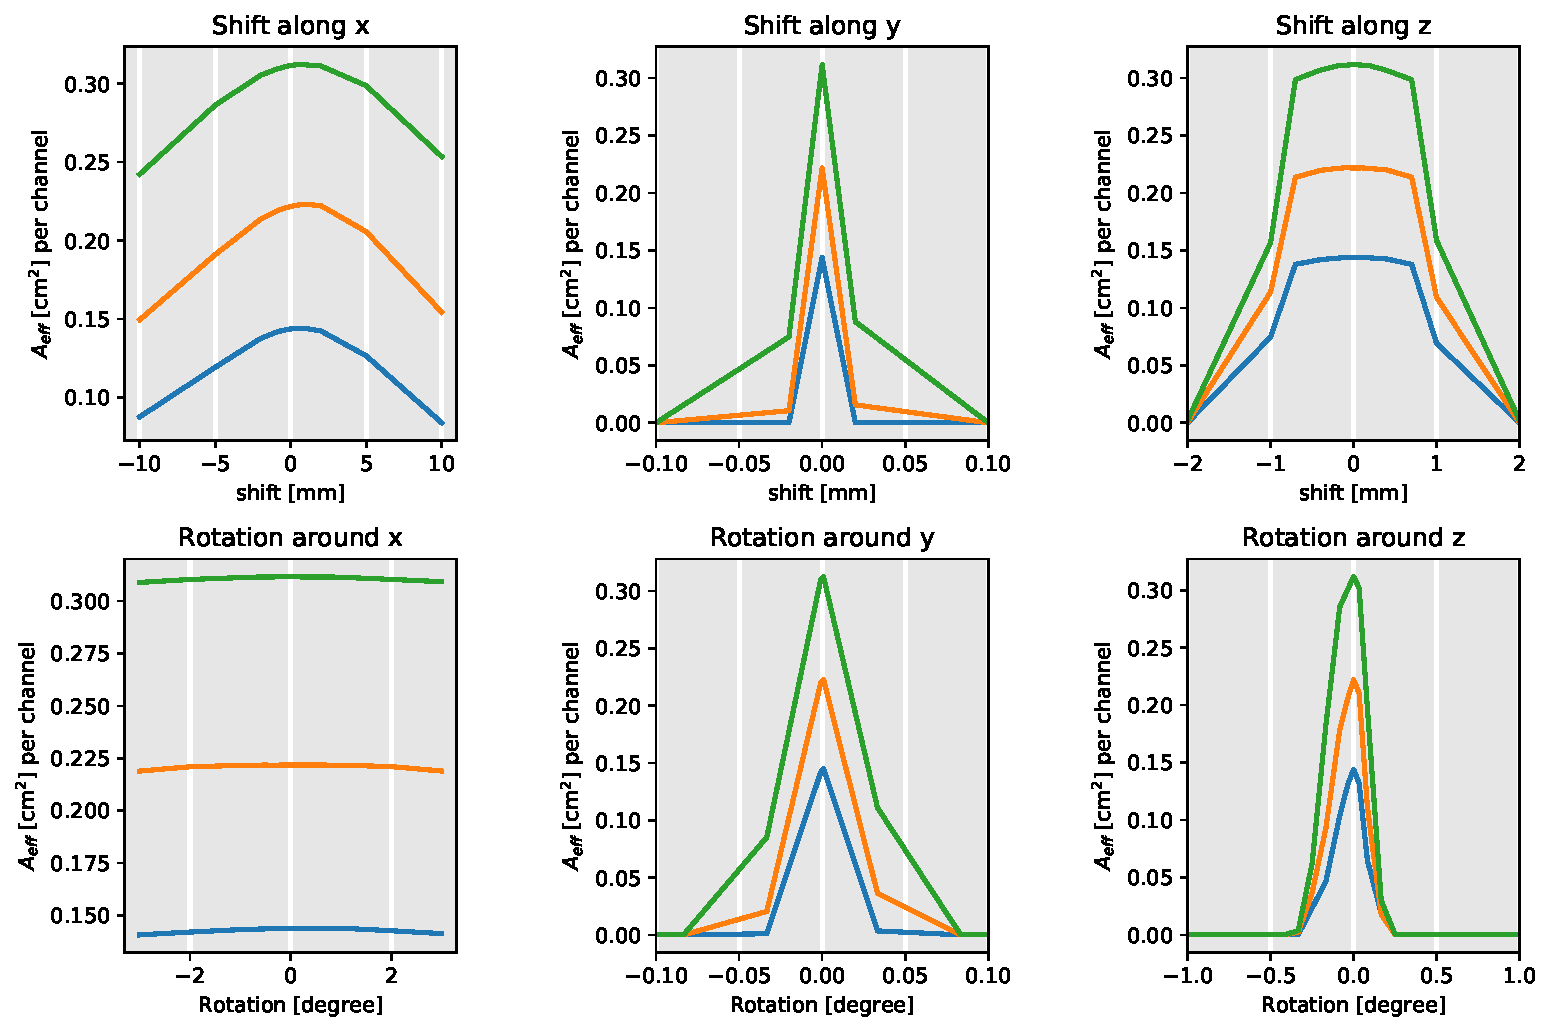
\includegraphics[height=8cm]{LGML_global.pdf}
  \end{center}
  \caption
      { \label{fig:LGML_global}Change of effective area in case of a misaligned ML mirror. 
}
\end{figure}

The ML is the most critical part of the alignment because photons have to hit the multilayer at the position of the Bragg peak. Because of this, shifts along the $y$ direction (the direction in which the multilayer is graded) are most sensitive (Figure~\ref{fig:LGML_global}) and have to be aligned to better than 10 micron. However, this is for a source at nominal position. Moving the source to a slightly off-axis position also changes where photons interact with the ML mirror. Thus, in practice, this alignment does not have to be performed to the 10 micron level for a single-channel instrument. Instead sources can just be observed slightly off-axis to compensate for any alignment error. This requires calibrating the alignment in space by observing a source at different positions, until the signal in the polarimetry channel is maximised. In this case, the instrument can no longer rotate around the nominal axis to probe different polarization angles. Instead, it has to rotate such that the source is kept at the new position determined in the calibration. On the other hand, tolerances for the other translations are a lot more relaxed around a mm or so.

However, for an instrument with more than one channel, the offset-pointing trick cannot be employed unless all ML mirrors are misaligned in exactly the same way.

Rotations around the long axis of the ML mirror ($x$ axis of the coordinate system) have a very large tolerance of a few degrees. Because the physical dimensions of the mirror are small, the point of intersection with the mirror surface does not change much and thus the photons still interact with the mirror very close to position of the Bragg peak. On the other hand, rotations around the other two axes move the mirror by a significant amount. That means that the photons travel either too far or too little and since the photons are dispersed, they will also travel to far or not far enough in $x$ direction, which causes them to miss the position of the Bragg peak and consequently reduces $A_{\mathrm{eff}}$ significantly.

\begin{figure} [ht]
  \begin{center}
    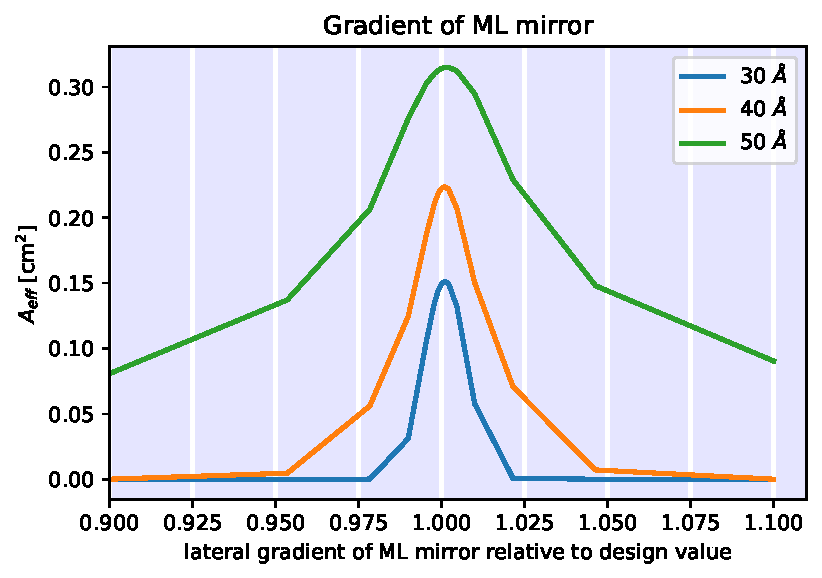
\includegraphics[height=5cm]{LGML_gradient.pdf}
  \end{center}
  \caption
      { \label{fig:LGML_gradient}Change of effective area for ML mirrors where the lateral grading differs from the design gradient.
}
\end{figure}

Another way for photons to miss the position of the Bragg peak is when the lateral grading of the ML mirror does not match the gradient that was assumed when placing the CAT grarings. Figure~\ref{fig:LGML_gradient} shows that the gradient has to be within about 1\% of the design value.

\subsection{Detectors}
The exact position of the detectors is not important as long as the signal still hits the detectors. With increasing misalignment, the spectral resolution of the polarimetry channel will degrade slightly, but the low signal in this channel will prevent an analysis of high-resolution spectroscopy anyway. Also, background also increases, when the extraction region size needs to be increased, but again, this effect is negligible for any misalignment that can reasonably be expected in the focal plane.

\section{SUMMARY}
One viable concept for a soft X-ray polarimeter is based on CAT gratings and a multi-layer mirror. We show ray-traces for an instrument designed for a small orbital mission with a focal length of 1.25~m and a single polarimetry channel. However, our results are easily generaliable to additional channels, since each channel acts essentially as its own instrument with separate CAT gratings, ML mirrors, and detectors. We show effective area and modulation factor based on this design.

Gratings need to be bend to mathc the blaze angle in a converging beam. We study different bending stategies and find that bending is required, but the performacne shows only little sensitivity to the exact value of the radius, so that only one type of grating holder with the same radius for all gratings is sufficient, simplifying design and handling. The requirement to place all gratings such that diffracted rays hit the ML mirror at the position of the Bragg peak puts limits on the size of the CAT gratings. We find that a width of 10~mm optimizes performance. 

Finally, we discuss alignment tolerances for all component. In most degrees of freedom the requirements are so loose that they are well below machining tolerances. One exception to that is the ML mirror, which has to be positioned with in 10~$\mu$m in dispersion direction.

\acknowledgments % equivalent to \section*{ACKNOWLEDGMENTS}       
Support for this work was provided in part through NASA grant NNX17AG43G and Smithsonian Astrophysical Observatory (SAO)
contract SV3-73016 to MIT for support of the {\em Chandra} X-Ray Center (CXC),
which is operated by SAO for and on behalf of NASA under contract NAS8-03060.
The simulations make use of Astropy, a community-developed core Python package
for Astronomy\cite{astropy1,astropy2}, numpy\cite{numpy}, and
IPython\cite{IPython}. Displays are done with mayavi\cite{mayavi} and matplotlib\cite{matplotlib}.


% References
\bibliography{report} % bibliography data in report.bib
\bibliographystyle{spiebib} % makes bibtex use spiebib.bst

\end{document} 
